\documentclass[]{article}
\usepackage{graphicx}
  \title{CDS 302 Final}
  \author{Sana Rehan}
  %\date{}

\begin{document}
\maketitle
\section{Schema diagram} 
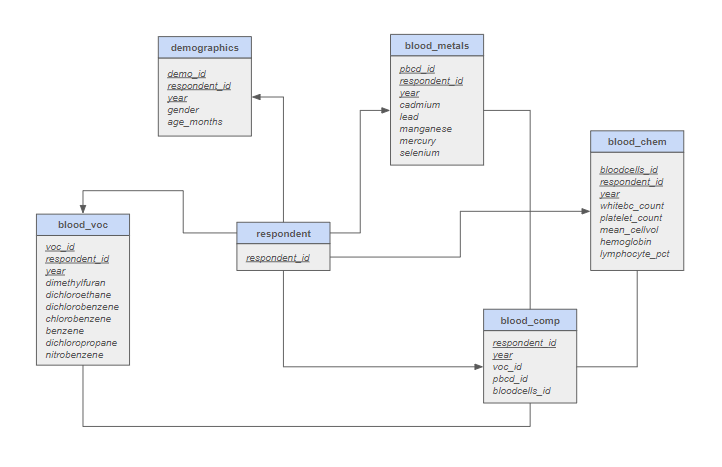
\includegraphics[scale=0.75]{relationaldiagram.png}

\section{Analysis}
The database was designed using data about blood from NHANES and contains five relations: \\
demographics(\underline{demo\_id}, \underline{respondent\_id}, \underline{year}, gender, age\_months) \\
bloodchem(\underline{bloodcells\_id}, \underline{respondent\_id}, \underline{year}, whitebc\_count, platelet\_count, mean\_cellvol, hemoglobin, lymphocyte\_pct) \\
blood\_metals(\underline{pcbd\_id}, \underline{respondent\_id}, \underline{year}, lead, cadmium, mercury, selenium, manganese) \\
blood\_voc(\underline{voc\_id}, \underline{respondent\_id}, \underline{year}, dimethylfuran, dichloroethane, dichlorobenzene, chlorobenzene, benzene, dichloropropane, nitrobenzene) \\
blood\_comp(\underline{respondent\_id}, \underline{year}, pbcd\_id, voc\_id, bloodcells\_id)

For my data analysis, I submitted 12 queries in total. 
I submitted a query to find the number of male and female respondents, respectively; aggregate function
The results were that the number of female respondents was 59262, and the number of male respondents was 57614. 

I submitted a query to find the minimum blood nitrobenzene level and the respondents associated with that level
The results were that the minimum blood nitrobenzene level was 0.0707, corresponding with respondents 21913, 23438, 24377, 24659, 35786, 26602, 28547, and 29326.

I submitted a query to find the maximum blood dimethylfuran level and the respondents associated with that value
The results were that the maximum dimethylfuran level is 1.45, and the respondent associated with that value is 85710.

I submitted a query to find the average blood selenium level for each set of years
The results were that the average blood selenium level for 2013-2014 was 159.466, for 2017-2018 was 167.304, for 2019-2020 was 159.466, for 2015-2016 was 159.567.

I submitted a query to find female respondents with blood lead levels above 0.5
The results were that the result was a table with the female respondents’ id numbers, the year, their gender, and their blood lead level. 

I submitted a query to find the average age of female and male respondents in years, respectively
The results were that the average age of female respondents was 16.020, and the average age of male respondents was 15.925. 

I submitted a query to find the average white blood cell count and average hemoglobin for each set of years
The result was a table with the years, and then the average white blood cell count and the average hemoglobin levels for each pair of years. The values were relatively consistent for each of the years, although there seemed to be a slight downward trend for average hemoglobin levels. 

I submitted a query to find all respondents with blood lead levels above 0.5 and their demographic information
The result was a table with the demographic information for each respondent who had blood lead levels above 0.5, as well as their blood lead levels. 

I submitted a query to find average lymphocyte percent for males and females, respectively
The results were that the average lymphocyte percent for females is 30.127%, and the average lymphocyte percent for males is 30.035%. 

I submitted a query to find blood metal content of all respondents whose blood benzene levels are above 0.3
The result was a table containing the gender, the age in months, the respondent\_id, and all of the blood metal information associated with that respondent\_id, of all respondents with blood benzene levels above 0.3. 

I submitted a query to find average platelet count of males and females, respectively
The results were that the average platelet count of females is 250.900, and the average platelet count of males is 231.683. 

I submitted a query to find demographic information about respondents whose blood lead levels are above 0.5 and whose blood mercury levels are above 0.3
The result was a table with the gender, the age in months, the blood lead level, the mercury level, as well as the demographic id, the respondent id and the year, of each respondent whose blood lead levels are above 0.5 and blood mercury levels are above 0.3. 

These queries demonstrate the ways that my database can allow healthcare researchers to utilize NHANES data about blood easily and efficiently. Additionally, I created a table that referenced several other tables by their primary keys in order to show the kinds of relations other researchers could make The NHANES data is difficult to process, since each year and each category is in a different XPT file, but this database streamlines access to the data and facilitates analysis. 


\end{document}